\chapter{Design}
\renewcommand{\baselinestretch}{\mystretch}
\label{chap:design}
\section{Overview}
The structure of this project is split into three sections; the device hardware, the device software, and host software. The device hardware is the organisation of the pre-built FPGA devices into a cluster configuration using custom inter-connectors for the cluster interface. The device software is the program that will be written onto each device and dictates their functionality. The device software comprises the bulk of the project, partitioning the computation into separate devices and handling all communication protocols between the devices. The host software runs on a host machine connected to the cluster and provides all source data for the system as well as receiving all the output data from the cluster system.


In this project the available hardware has been the motivating design limitation, and so discussion of the hardware configuration is discussed first, the characteristics of which will motivate the design decisions made in the rest of the design.

%\setlength{\parindent}{0pt}
\section{Hardware}
The motivation of this project was a scalable system and the design of the HDL is intended to be built such that it can be implemented on any FPGA hardware with the relevant ports. For the purposes of testing in this project three DE0 FPGAs will be used (shown in Figure \ref{fig:de0}).


The Terasic DE0 board contains an Altera CYCLONE III FPGA with 15,408 logic elements and 512kb of memory. This chip is capable of hosting around 9 pixels from the original algorithm within around 10 000 logic elements. This board has a relatively large number of general purpose input/output ports with 2 40-pin connectors on the side of the board. It also has a 5-pin RS232 specification UART which may be used for host computer to device simulation. 

In order to  ensure that the design of the system is scalable to other architectures and interfaces, the UART controller can be logically partitioned and replaced in other applications as will be discussed in the HDL design.  First estimates of the number of interconnect ports needed are around 40 pins minimum with the scaling as the design parameters change. As these FPGA development boards are available freely within the department they will be used for the prototype system design. It is important to note however, that this should not impact the design in such a way that stops the design from being easily moved to other boards when necessary. A secondary benefit of this board is the large number of user input/output ports such as 4 7-segment displays which can be used for debugging and progress checking.  This board was freely available within the department and therefore made a good low cost prototyping unit, however these boards can be bought at a retail price of \$120. 


\begin{figure}[h!]
  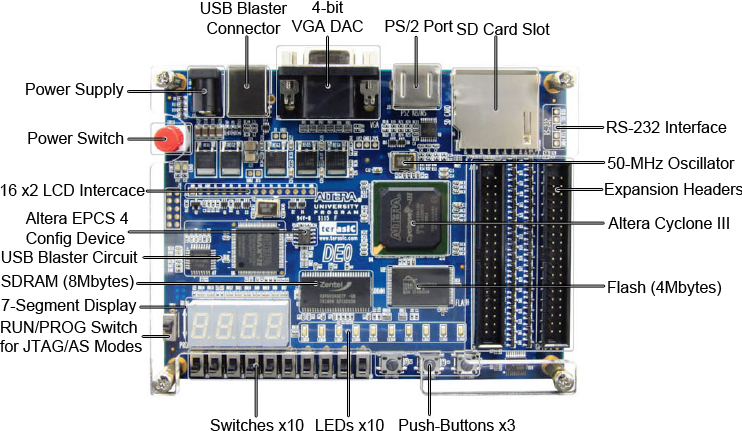
\includegraphics[width=\textwidth]{./figs/de0.png}
  \caption{Terasic DE0 FPGA Board}
  \label{fig:de0}
\end{figure}


An important decision to be made in the design of the hardware was whether to use a common clock across all the devices, or to use separate clocking. The advantage of the single clock is that the processors can work in lock-step reducing communication delays and simplifying the interconnect protocol. However, a common clock places other limitations on the design. The common clock design limits the clock frequency of all the devices to the speed at which the inter-FPGA communication can happen, this may lower the theoretical maximum clock speed, however the design already runs at a relatively low clock speed and the intentional is to overcome this limitation with parallelisation. The common clock will need to be considered in the testing stage, as identifying the clock speed where correct operation is primarily done through trial and error with a trade-off between bit-error rates and speed. The ring network design of this system favours the common clock approach as all communication is exclusively done with nearest neighbours, limiting the length of the inter-FPGA communications. 

\subsubsection{Inter-Device Communication Hardware}
All inter-FPGA communications will be done using the 40-pin GPIO connectors that were discussed earlier. The communication is done exclusively in a ring, which lends itself to a dual connector geometry. For each device the second GPIO connector will be linked to the first GPIO connector of the next device, with the final device looping back to the first connector of the first device. This is better than all-to-all communication, as that would scale extremely badly with number of devices as well as using far more ports. This takes care of the communication, however it is also necessary to have a shared global clock. This is achieved by separating one of the wires from the ribbon cable that connects the GPIO and connecting it together. This design is shown in figure \ref{fig:interfpga}, and is shown implemented on the board in the implementation section, figure \ref{fig:cluster}. The practical applications of this is also considered in the implementation section where the speed of the connection is analysed. 

\begin{figure}[h!]
  \includegraphics[width=\textwidth]{./figs/interfpga.pdf}
  \caption{Inter-FPGA Communication Hardware Setup}
  \label{fig:interfpga}
\end{figure}

\subsubsection{UART Hardware}
The UART interface on the board is theoretically designed to interface with any other RS232 standard UART controller, and the data streaming protocol will be covered in the Device Software section. For the purposes of interfacing with a host computer a USB to UART cable has been bought. Capable of up to 1~Mbaud the FTDI USB-RS232, this cable allows communication between the host software and device software using a virtual COM port for which there are multiple Application Programming Interfaces (APIs) available. The 1~MBaud limit allows up to 921,600 bits per second to be transmitted, when this is considered in the scope of the streaming project where each pixel has  a 2 bit data sample taken in the order of seconds and a DE0 FPGA can fit around 10 Pixels per device, the data rates this interface is capable of far exceed the rates needed. Only when devices with hundreds of pixels are present or extremely large arrays of devices are used will this present a problem. On the DE0 board a level shifter is present, this turns the 3.3v device signals into the $\pm$13v standard that RS232 uses.
 %hardware
\section{Device Software}




\subsection{Overview}

The device software makes up the bulk of the work done within this project. The basic algorithm devised by Y Hu et al is mostly unmodified, with the modifications limited primarily to the communication of data between devices. This work can broadly be split into three sections; the data input handler, the inter-FPGA communication, and the library data read-out. The data input handler interfaces with the host software and distributes the input data across the system. The inter-FPGA communication controls the algorithm's execution to guarantee synchronisation across the multiple devices. The result data handler returns the overlap libraries produced by each pixel via the UART interface with the host. In order to explain the design of these three sub-systems it is important to understand the over-arching aims of the device software. The top level of this system can be seen in figure  \ref{fig:tld}. Each device contains a data Input/Output (IO) handler as well as small modifications to the global controller. Through maintaining the same structure as far as possible, the implementation minimises the impact of cross-device interfacing on each device's operations.

What this approach does in terms of the algorithm is split work in a uniform fashion, increasing the work done by a single pixel, but keeping the total work done per FPGA the same. This can be explained by viewing an all-against-all comparison as a matrix of comparisons.




$
\text{Comparison Matrix} =  
\begin{pmatrix}
  F(a_{1},a_{1}) & F(a_{1},a_{2})  & \cdots & F(a_{1},a_{n}) \\
  F(a_{2},a_{1}) & F(a_{2},a_{2})  & \cdots & F(a_{2},a_{n}) \\
  \vdots  & \vdots   & \ddots & \vdots   \\
  F(a_{n},a_{1}) & F(a_{n},a_{2}) & \cdots & F(a_{n},a_{n}) \\
 \end{pmatrix}  
 $
 
 
Within this matrix each pixel does one column of work, performing the comparison between 1 common sequence and all other sequences. However, there are no true dependencies within this matrix, any comparison can be carried out in any order. In the original comparison engine, the movement of data around the chip was the driving factor, so each pixel started with it's own sequence, and then used data forwarded around the ring network. This can be understood within the matrix as each pixel starting on it's entry in the leading diagonal of the matrix and then working up the matrix, looping at the top down to the bottom. In this way all the comparisons happen together in lockstep.

Splitting this algorithm across mutliple devices is complex due to this fact however, as currently pixels only do the same number of comparisons as there are on the board. In the newer design one of these pixels will still do the comparisons with all the sequences from the entire cluster, and as such the link between number of pixels present and  number of comparison cycles must be broken. Each device can then be viewed as a rectangular matrix, which when concatenated form the previous complete matrix as shown below for 3 devices.




\begin{align*}
\text{FPGA}_0
 &=
 \begin{pmatrix}
  F(a_{1},a_{1}) & F(a_{1},a_{2})  & \cdots & F(a_{1},a_{\frac{n}{3} }) \\
  F(a_{2},a_{1}) & F(a_{2},a_{2})  & \cdots & F(a_{2},a_{\frac{n}{3} }) \\
  \vdots  & \vdots & \ddots & \vdots   \\
  F(a_{n},a_{1}) & F(a_{n},a_{2})  & \cdots & F(a_{n},a_{\frac{n}{3} }) \\
 \end{pmatrix} \\
\text{FPGA}_1
 &=
 \begin{pmatrix}
  F(a_{1},a_{\frac{n}{3}+1}) & F(a_{1},a_{\frac{n}{3}+2})  & \cdots & F(a_{1},a_{\frac{2n}{3}}) \\
  F(a_{2},a_{\frac{n}{3}+1}) & F(a_{2},a_{\frac{n}{3}+2})  & \cdots & F(a_{2},a_{\frac{2n}{3}}) \\
  \vdots  & \vdots & \ddots & \vdots   \\
  F(a_{2n},a_{\frac{n}{3}+1}) & F(a_{n},a_{\frac{n}{3}+2})  & \cdots & F(a_{n},a_{\frac{2n}{3}})
 \end{pmatrix} \\
 \text{FPGA}_2
 &=
 \begin{pmatrix}
  F(a_{1},a_{\frac{2n}{3}+1}) & F(a_{1},a_{\frac{2n}{3}+2})  & \cdots & F(a_{1},a_{n}) \\
  F(a_{2},a_{\frac{2n}{3}+1}) & F(a_{2},a_{\frac{2n}{3}+2})  & \cdots & F(a_{2},a_{n}) \\
  \vdots  & \vdots & \ddots & \vdots   \\
  F(a_{2n},a_{\frac{2n}{3}+1}) & F(a_{n},a_{\frac{2n}{3}+2})  & \cdots & F(a_{n},a_{n})
 \end{pmatrix} \\
 \\
\text{Comparison Matrix} &= \text{FPGA}_0 \parallel \text{FPGA}_1 \parallel \text{FPGA}_2 \\
\end{align*} 


This shows there are now $\frac{n}{y}$ pixels per device with y devices, but each pixel still does n comparisons. This idea will be revisited later in discussions of other future work.
 
The decision was made to favour a shared clock, lockstep operation design for this implementation, the reason for this is that the ring network design has a natural dependancy loop. This would mean any discrepancy in throughput would cause the system to  hang both for the slowest element of the system but also for communication within the system and would require significant local data storage to mitigate local sources of latency such as long memory accesses on a single FPGA. The lock step design introduces a problem of both guaranteeing coherence across the system as well as practical limitations on clock speed. These practical limitations will be discussed in the implementation section.



The algorithm provided gives a number of important features that must be kept, stream processing and independent logical elements being the most important. 
\begin{sidewaysfigure}[p]
  \centering
  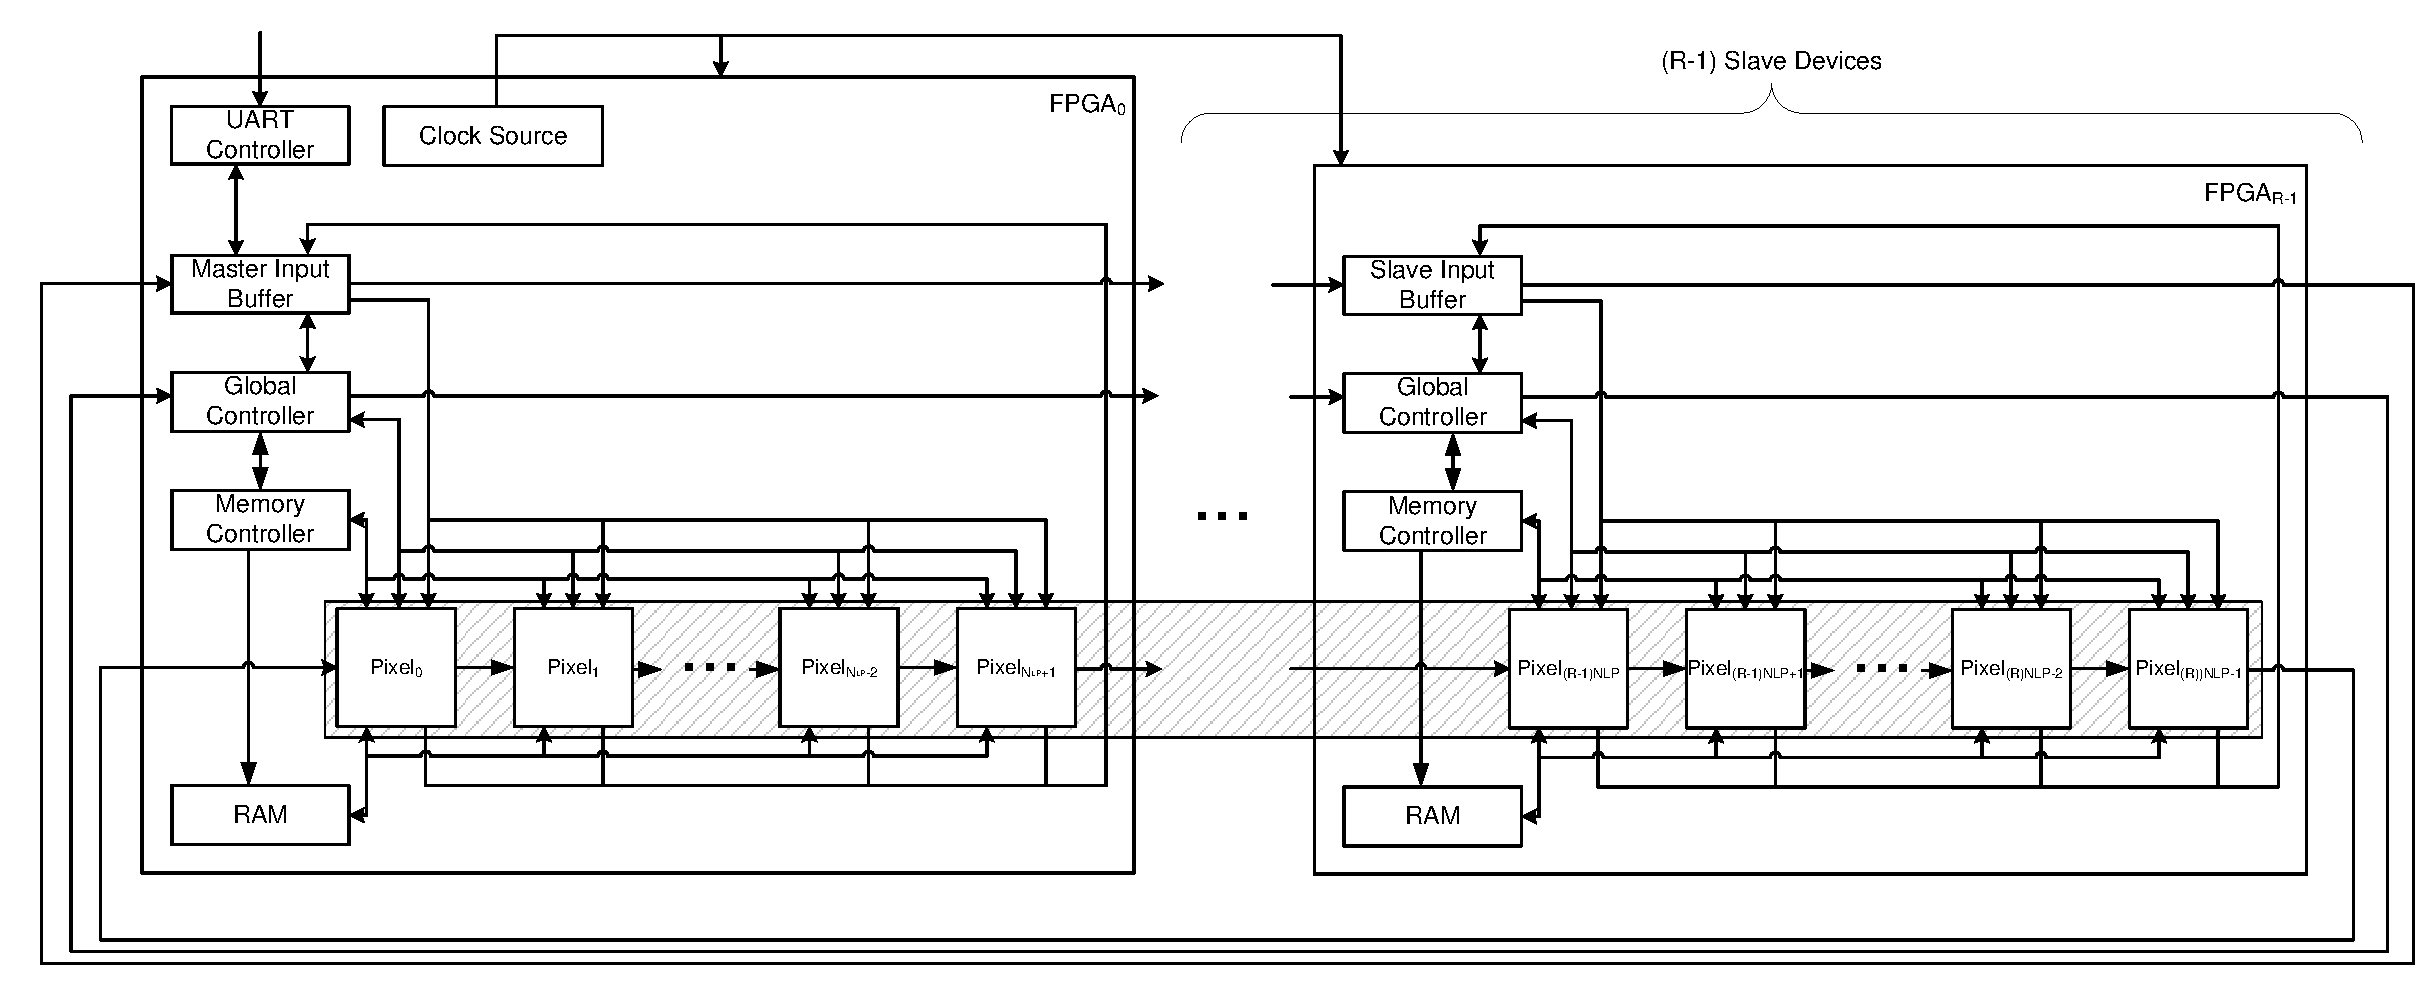
\includegraphics[width=\textheight]{./figs/MFPGA.pdf}
  \caption{Top Level Diagram, 1 Host, R-1 Slave Devices}
  \label{fig:tld}
\end{sidewaysfigure}


\subsection{Data Input Handler}
All the data transfers with the host machine are done via one connection, this is present only on a master FPGA, the other devices received data forwarded around the ring network. It is important however, that the processing happens in lock step, as a result the input data must be available on all FPGAs at the same time. This can be done either through communication between FPGAs or through strict control of the data path. As communication is relatively expensive (due to the high latency of sending signals around the ring network) a fixed latency approach has been chosen. As an over-arching design decision, all signals sent between devices are clocked out and in with no logic. This guarantees the maximum allowance for the data path between devices. 

\subsubsection{The Master UART Connection}
Present only on the master device, the UART interface works at the $\pm$13~volt RS232 specification with the data transfer protocol shown in figure \ref{fig:UART}. The UART controls both the incoming data to be processed and the outgoing data reported to the host. The format of the incoming data is a stream ordered first by read order then by pixel order. The data rate achieved by this interface is up to 1~Mbaud, this is 1 million symbols per second. In the context of  a device that can fit up to 100 pixels as discussed in the complexity analysis of the algorithm, this is significantly faster than necessary. The primary goals of the UART connection is fast enough data rates with low error rates. This is achieved with the oversampled interface. This means for a 1~MBaud system running on  a device with a faster clock, each data bit is sampled multiple times, thus reducing error rates. 
\begin{figure}[!h]
  \centering
  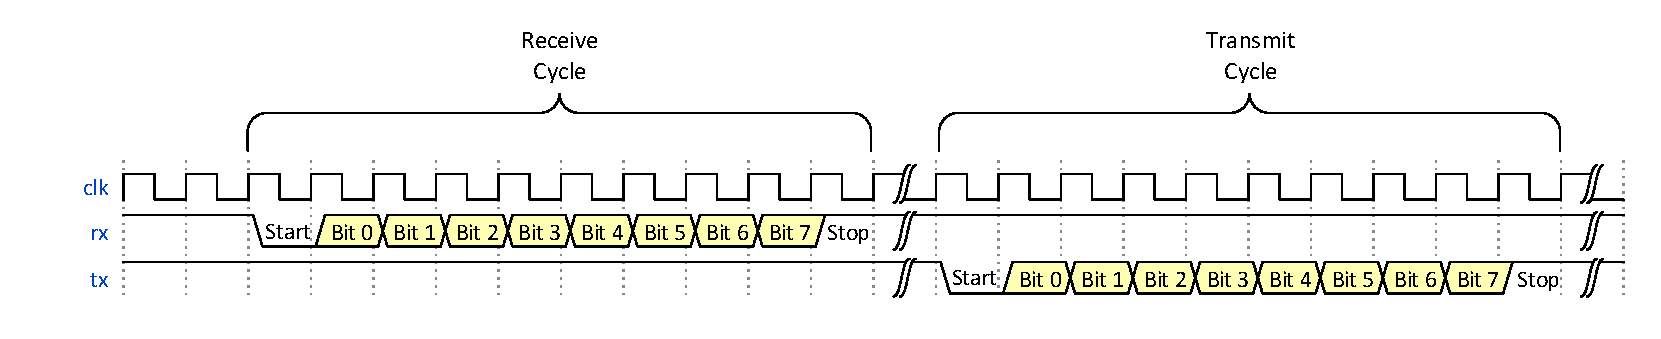
\includegraphics[width=\textwidth]{./figs/UART.pdf}
  \caption{UART Interface Protocol}
  \label{fig:UART}
\end{figure}


The UART controller on the device is designed as a separate module with a simple interface. The reason for this is that if necessary, different external interfaces can replace the UART if necessary. This would be common when implementing the design different hardware which may only have connections for protocols like USB or PCI-Express. In the case of this project an external piece of code was used to interface with the UART standard, this was done as UART interfaces are a standard piece of code and there is little value in reproducing this work.


\subsubsection{Distribution of Input Data}
\begin{figure}[!h]
  \centering
  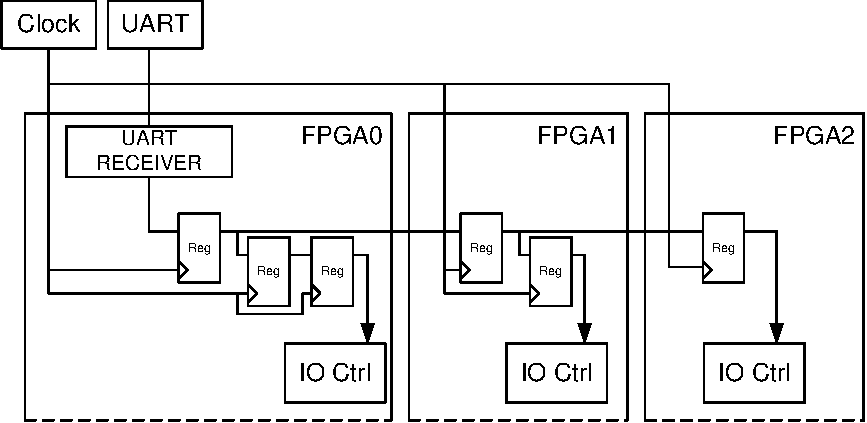
\includegraphics[width=0.8\textwidth]{./figs/input_delay.pdf}
  \caption{Input Delay System Example for 3 Devices}
  \label{fig:delay}
\end{figure}
One of the keys to the lock-step design is ensuring that all the input data appears available to the processor across all devices at the same time. This can be ensured by a simple system of delay registers. This system is shown in figure \ref{fig:delay}, it ensures that all FPGA input adaptors receives the data in lock step. Technically this requires the forwarding of more data than necessary, as data for all pixels reach all FPGAs, as well as invalid data being forwarded with an invalid flag. However, removing this redundancy could not shorten the delay and complicates the logic so it was decided to be preferable to complex logic. The output of this delay cycle is identical across all devices, an 8 bit data chunk with a valid signal going in to the data format translator. The result of this process is a latency of N cycles, where N is the number of devices in the cluster. It is important to note that latency is not an issue in terms of the end speed of the cluster, as it will be hidden during the processing time and is relatively negligible. 






\subsubsection{Data Format Translation}
As discussed earlier, the UART used to input data (and the interface to forward the data between FPGAs) consists of a byte based transmission system. This means data comes in 4 pixels at a time, however the system requires 2 bits to be sent to each pixel in parallel. This requires a complex data width adaptation. This is achieved by clocking data into a wide register 8 bits at a time, and then writing it out to a First In First Out (FIFO) memory structure at the correct bit width. The memory structure adds a small amount of processing flexibility in the case that data is coming in faster than can be processed. In this project the FIFO can store all input data, this is possible due to the fact the comparison engine is very logic element intensive but not memory intensive. A correctly designed FIFO maps to a memory bits on chip, a separate resource to the logic utilisation. As discussed earlier, for a 9 pixel design over 80\% of the logic elements are used on a DE0 device, but less than 1\% of the memory is used. The translation system is a relatively complex translation as is shown in figure \ref{fig:translator}. It is important to note that this width adaptor requires more than 1 pixel per device, otherwise the input adaptor register will be overwritten by a single input twice in a single cycle.

\begin{figure}[!h]
  \centering
  \includegraphics[width=0.9\textwidth]{./figs/input_adaptor.pdf}
  \caption{Input Adaptor, N$_{LP}$-Number of Local Pixels, N$_{TP}$-Number of Total Pixels}
  \label{fig:translator}
\end{figure}



\subsection{Inter-FPGA Communication}

Inter-FPGA communication provides both algorithm synchronisation and extension of the ring network. As shown in figure \ref{fig:tld} the global controller on each device communicates and the ring network communicates.

The extension of the ring network is the most simple, the communication that would normally happen forwarding suffix data between pixels is routed across the GPIO ports as described in the hardware section. Algorithmically this is identical to the original implementation but limits the clock speed due to data transfer rates. This interface is an important limiting factor for the design. The number of connectors between the devices for the ring network is 4 bits for every parallel string being forwarded, this quickly reaches the limits of the number of connectors available. 


The global controller interface is more complex due to the non-fixed nature of the state machine. The state machine for the original algorithm is shown in figure \ref{fig:ctrlfsm}. It can be seen, the only conditional transitions are on input data being available, and checking for pixels to complete. The other transitions are all determined by fixed length states. 


\begin{figure}[!h]
  \centering
  \includegraphics[width=\textwidth]{./figs/ctrl_fsm.pdf}
  \caption{Algorithm Global Controller Finite State Machine}
  \label{fig:ctrlfsm}
\end{figure}


The transition for moving into the read state is conditional on the data being available, as is covered in the previous section, measures have been taken to ensure this happens identically on all devices. The transition from the Wait for All state to Idle state is more difficult however. All pixels must report ready to the controller before the state can proceed. This is very difficult to do across several FPGAs fast, so instead a distributed mechanism has been designed. Each device has all it's pixels report, when all pixels on the master report  it forwards a done signal. Each slave then forwards this signal only when its own pixels are done. When the master receives the done signal back, it then sends a proceed signal and waits a fixed length of time, each slave forwards this signal immediately and waits for 1 fewer cycles. In this way it is guaranteed they count down together. Finally at the end of the countdown they proceed to the next step.

The net result of this in terms of cycles per comparison is that one cycle through the state machine (which corresponds to 1 new piece of data) is increased by $2 \times $the number of pixels. This protocol lowers the speed of comparisons in cycle count, but allows for the fast shared clock. The impact of this will be studied in the testing and evaluation sections. 





\subsection{Result Data Handler}

The result data in the algorithm is stored on a per pixel basis in a library of complex data structures. This library is shown in the listing below. These library entries are known as overlap seeds.


 \begin{center}

 \begin{minipage}{\textwidth}
\lstset{language=python, numbers=left, showspaces=false,
    showstringspaces=false, tabsize=4, breaklines=true, captionpos=b, numbersep=5pt }
\begin{lstlisting}[frame=single,caption=Result Data Format, label=listing:record]
	TYPE SEED IS RECORD
		posi   : RD_INT_TYPE; -- range 0 to READ_LENGTH
		rota   : PIXEL_INT_TYPE; --range 0 to PIXEL_COUNT
		score  : EDDI_INT_TYPE; -- range 0 to REDUNDANCY + 1
		chk_wt : WAIT_INT_TYPE; -- range 0 to INFIX_LENGTH
		bases  : BASE_VECT; -- array 0 to 2 REDUNDANCY + 1
		lock   : STD_LOGIC; 
	END RECORD;
\end{lstlisting}
 \end{minipage}
\end{center}
This data structure is highly dependant on the parameters of the comparison engine and therefore the size is variable. Each library has a parameterisable number of entries and there is one library per pixel. To write this data out across the UART 3 processes must take place. First the data must be gathered per deice and formatted for transfer, then the data must be gathered on the master device, finally the data must be sent out across the UART.
\begin{figure}[!h]
  \centering
  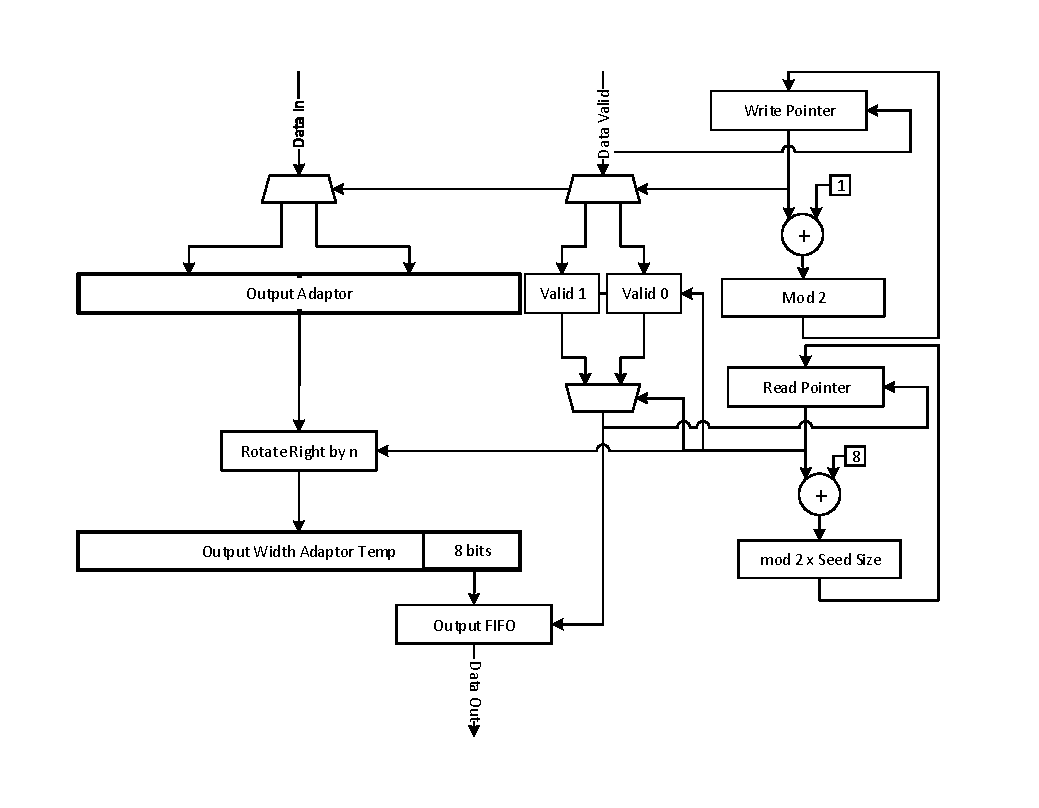
\includegraphics[width=\textwidth]{./figs/output_adaptor.pdf}
  \caption{Output Width Adaptor}
  \label{fig:owa}
\end{figure}

The first stage requires the record to be flattened into a single vector data type. The IO controller on each device then cycles through each pixel requesting their records until they report the end. This then creates a local copy of the libraries together, however this is formed of very large data types that are not suitable for transferring off-chip. Another data width adaptation is required to allow communication between devices, shown in figure \ref{fig:owa}. 


Having translated the current library data into a transferrable format this has to transferred across the ring network. Inter-FPGA communication is already quite high, requiring a large amount of connections so it is best to re-use the data forwarding connections that were used for the input data. The time multiplexing of this connection can safely be used with no effect on performance. The data on the ring network must be transferred in a fixed order to allow reconstruction of the library on the host, this is done by transferring all data from the first slave, followed by an end signal. Each slave in the network forwards the data and uses the stop signal as a prompt to append their own data. The master FPGA caches this data and transmits it over UART, appending it's own library. The impact of caching the full library on one device is small. As covered earlier, memory usage is already extremely low and the library data by nature is only a small fraction of the input data.



 %software
\section{Host Software}
One of the stated goals of this project was to produce a real-time system and a suggested way to achieve this was through the use of a streaming interface between the DNA detection hardware and assembly algorithm. Compatability with this goal is covered in the device software section of the report covering the UART streaming interface. However, for the purposes of this report and for testing and verification of the project the host software built here will use a fixed data source with generated test data. 

In order to simplify the host side interface with the device software an FTDI cable was used (as covered in the Device Hardware section). The host software has two simple functions, to read data from a text file and transmit it to the UART, and read result data from the UART out to another text file. In order to maximise backwards compatibility and ease of testing, I will adopt the formatting of the input data used by Y Hu in his test bench for the original algorithm. This consists of N lines of M length, where N is the number of pixels and M is the read length, the DNA bases are represented by capital letters; A- Adenine, T- Thymine, C- Cytosine and G- Guanine. An example input file is shown in \ref{listing:example}. This format is a standard format used in a number of tools including the ABySS sequencer and the BLAST sequencer \cite{ABySS}\cite{BLAST}. \\


\begin{minipage}{0.8\textwidth}

\begin{center}

 \lstset{numbers=left, showspaces=false, showstringspaces=false, tabsize=4, basicstyle=\tt, breaklines=true, captionpos=b, numbersep=5pt }
\begin{lstlisting}[ frame=single,caption=Input Data Format Example; 9 Pixels\, Read length 50, label=listing:example]
 CGAGGGATGTCTCTTGCGTGTCAAACAACTCTCTTTCGTTACTATGCGGG
 AATTCGTATCAACATATGTCGGGGTTCATATGGACACTATAGGCAGGTGT
 AGATAGCCGTTTCGAAGTTGAATGACTGTGCCCAGAACGTACTCAGATCC
 AGACAGCATCAAAGCACACTATTCCCGACCGTAGGGACCTAACGGATTAG
 ATCGTAGAACCCGAAGACGGAGTTCCCGTAATAGAGCCAAAGTATGTTGT
 ACACGTGTCTAGCACGGCAAACGGGCCAGGGTCCCTATGGGTAAGGACCG
 GTCATGCGCCCGTTGAAGGCTTAGTCTAAATTGTATTTAGCACCATGGCT
 GGATTAAATGCGCATGCAACGGATACTGAACATGGGCAATACGCGTTAAC
 GACCCGAAGGTTTTCGGCTGCGACTCCAACGACCGTCTGTAGGCTGGATT
\end{lstlisting}

\end{center}
\end{minipage}

In order to make this compatible with the streaming interface, this input data must then be converted to binary and re-ordered. The binary translation for each base is as follows: A: 00, T: 01, C: 10, G:11. The streaming interface requires that the data is transferred ordered first by read number, then by pixel count. This translation is done by the code listed in Appendix \ref{App:Host_Software}

Similarly the host software is required to unpack the output data from the FPGA, this is also done through simple python bit manipulation and writes the output to a file, ordering the library data in the same format as it is present on the FPGA local memory. This can then be used to carry out a comparison with the simulated data in the test bench setting or used to recombine the data in a true application of the algorithm. 

This functionality is achieved through a python script that can be run from the command-line, passing in the parameters dictating read length, pixel count and the location of the source data. This script automatically interfaces with the device and prints the result data to a timestamped text file in the destination directory. This code is included in appendix \ref{App:Host_Software} and a guide how to use this is included in the user guide appendix \ref{App:UserGuide}.
\vspace*{\fill} %Host Software